% -----------------------------------------------
% Template for ISMIR 2014
% (based on earlier ISMIR templates)
% -----------------------------------------------

\documentclass{article}
\usepackage{graphicx,psfrag,pstricks,epsf,url}
\usepackage{ismir2014,amsmath,cite}
\usepackage{subfigure}
\usepackage{amsfonts}
% For citations
%\usepackage{natbib}
% For algorithms
\usepackage{algorithm}
\usepackage{algorithmic}

% Title.
% ------
\title{RNN-based Music Language Models for Improving Automatic Music Transcription}

% Single address
% To use with only one author or several with the same address
% ---------------
%\oneauthor
% {Names should be omitted for double-blind reviewing}
% {Affiliations should be omitted for double-blind reviewing}

% Two addresses
% --------------
%\twoauthors
%  {First author} {School \\ Department}
%  {Second author} {Company \\ Address}

% Three addresses
% --------------
\threeauthors
  {First author} {Affiliation1 \\ {\tt author1@ismir.edu}}
  {Second author} {\bf Retain these fake authors in\\\bf submission to preserve the formatting}
  {Third author} {Affiliation3 \\ {\tt author3@ismir.edu}}

% Four addresses
% --------------
%\fourauthors
%  {First author} {Affiliation1 \\ {\tt author1@ismir.edu}}
%  {Second author}{Affiliation2 \\ {\tt author2@ismir.edu}}
%  {Third author} {Affiliation3 \\ {\tt author3@ismir.edu}}
%  {Fourth author} {Affiliation4 \\ {\tt author4@ismir.edu}}

\begin{document}
%
\maketitle
%
\begin{abstract}
In this paper, we investigate the use of Music Language Models (MLMs) for improving Automatic Music Transcription performance. The MLMs are trained on sequences of symbolic polyphonic music from the Nottingham dataset. We train Recurrent Neural Network (RNN)-based models, as they are capable of capturing complex temporal structure present in symbolic music data. Similar to the function of language models in automatic speech recognition, we use the MLMs to generate a prior probability for the occurrence of a sequence. The acoustic AMT model is based on probabilistic latent component analysis, and prior information from the MLM is incorporated into the transcription framework using Dirichlet priors. We test our hybrid models on a dataset of multiple-instrument polyphonic music and report a significant 3\% improvement in terms of F-measure, when compared to using an acoustic-only model.

% In this paper, we investigate the use of Music Language Models (MLMs) for improving Automatic Music Transcription (AMT) performance. AMT is the process of converting an acoustic music signal into a symbolic notation, and is considered to be a fundamental problem in music signal processing. The MLMs are trained on sequences of symbolic polyphonic music. We train Recurrent Neural Network (RNN)-based models, as they are capable of capturing complex temporal structure present in symbolic music data. Similar to the function of language models in automatic speech recognition, we use the MLMs to generate a prior probability for the occurrence of a sequence. The acoustic AMT model is based on probabilistic latent component analysis, and prior information from the MLM is incorporated into the transcription framework using Dirichlet priors. We test our hybrid models on a dataset of multiple-instrument polyphonic music and report a significant 3\% improvement in terms of F-measure, when compared to using an acoustic-
% only model.
\end{abstract}
%


\section{Introduction} 
\label{sec:introduction}

Automatic Music Transcription (AMT) involves automatically generating a symbolic representation of an acoustic musical signal \cite{Benetos2013b}. AMT is considered to be a fundamental topic in the field of music information retrieval (MIR) and has numerous applications in related fields in music technology, such as interactive music applications and computational musicology. %Typically, the output of an AMT system is a \textit{piano-roll} representation, which is a two-dimensional matrix representation of a musical piece where the X-axis represents time quantized into regular intervals, and the Y-axis represents the keys of a piano in increasing pitch. A cell in this matrix is $1$ if the key represented by its Y-coordinate is sounding at the time instant represented by its Y-coordinate.
The majority of recent transcription papers utilise and expand \emph{spectrogram factorisation} techniques, such as non-negative matrix factorisation (NMF) \cite{Li1999} and its probabilistic counterpart, probabilistic latent component analysis (PLCA) \cite{Smaragdis2006}. Spectrogram factorisation techniques decompose an input two-dimensional spectrogram of the audio signal into a product of spectral templates (that typically correspond to musical notes) and component activations (that indicate whether each note is active at a given time frame). Spectrogram factorisation-based AMT systems include the work by Bertin et al.\ \cite{Bertin2009}, who proposed a Bayesian framework for NMF, which considers each pitch as a model of Gaussian components in harmonic positions. Benetos and Dixon \cite{Benetos2012} proposed a convolutive model based on PLCA, which supports the transcription of multiple-instrument music and supports tuning changes and frequency modulations (modelled as shifts across log-frequency). 

In terms of connectionist approaches for AMT, Nam et al. \cite{Nam2011} proposed a method where features suitable for transcribing music are learned using a deep belief network consisting of stacked restricted Boltzmann machines (RBMs). The model performed classification using support vector machines and was applied to piano music. B\"{o}ck and Schedl used recurrent neural networks (RNNs) with Long Short-Term Memory units for performing polyphonic piano transcription \cite{Bock2012}, with the system being particularly good at recognising note onsets. 

There is no doubt that a reliable acoustic model is important for generating accurate symbolic transcriptions of a given music signal. However, since music exhibits a fair amount of structural regularity much like language, it is natural for one to think of the possibility of improving transcription accuracy using a \textit{music language model} (MLM) in a manner akin to the use of a language model to improve the performance of a speech recognizer \cite{Rabiner1993}. In \cite{Boulanger-Lewandowski2012}, the predictions of a polyphonic MLM were used to this end, which was further developed in \cite{Boulanger-Lewandowski2013}, where an input/output extension of the RNN-RBM was proposed that learned to map input sequences to output sequences in the context of AMT. Both in \cite{Boulanger-Lewandowski2012} and \cite{Boulanger-Lewandowski2013}, evaluations were performed using synthesized MIDI data. In \cite{Raczynski13}, Raczy\'{n}ski et al. utilise chord and key information for improving an NMF-based AMT system in a post-processing step.

%Another example of symbolic information which can improve the performance of acoustic models are \textit{score informed} approaches, which have been applied in music research tasks, e.g. for tonic identification \cite{Senturk2013}. % More references, if required: Source separation - Ganseman2010, Hennequin2011

In the present work, we integrate a MLM with an AMT system, in order to improve transcription performance. Specifically, we make use of the predictions made by a Recurrent Neural Network (RNN) and a Recurrent Neural Network-Neural Autoregressive Distribution Estimator (RNN-NADE) based polyphonic MLM proposed in \cite{Boulanger-Lewandowski2012} to refine the transcriptions of a PLCA-based AMT system \cite{Benetos2012, Benetos2013}. Information from the MLM is incorporated into the PLCA-based acoustic model as a prior for pitch activations during the parameter estimation stage. It is observed that combining the two models in this way boosts transcription accuracy by +3\% on the Bach10 dataset of multiple-instrument polyphonic music \cite{Duan2010}, compared to using the acoustic AMT system only.

The outline of this paper is as follows. The PLCA-based transcription system is presented in Section \ref{sec:transcription}. The RNN-based polyphonic music prediction system that is used as a music language model is described in Section \ref{sec:prediction}. The combination of the two aforementioned systems is presented in Section \ref{sec:combination}. The employed dataset, evaluation metrics, and experimental results are shown in Section \ref{sec:evaluation}; finally, conclusions are drawn in Section \ref{sec:conclusions}.

\section{Automatic Music Transcription System} \label{sec:transcription}


For combining acoustic and music language information in an AMT context, we employ the model of \cite{Benetos2012}, which supports the transcription of multiple-instrument polyphonic music and also supports pitch deviations and frequency modulations. The model of \cite{Benetos2012} is based on PLCA, which is a latent variable analysis method which has been used for decomposing spectrograms \cite{Shashanka2008}.
%and can be viewed as a probabilistic version of non-negative matrix factorization \cite{Li1999}. 
For computational efficiency purposes, we employ the fast implementation from \cite{Benetos2013}, which utilized pre-extracted note templates that are also pre-shifted across log-frequency, in order to account for frequency modulations or tuning changes. In addition, as was shown in \cite{Smaragdis2009}, PLCA-based models can utilise priors for estimating unknown model parameters, which will be useful in this paper for informing the 
acoustic transcription system with symbolic information.

The transcription model takes as input a normalised log-frequency spectrogram $V_{\omega,t}$ ($\omega$ is the log-frequency index and $t$ is the time index) and approximates it as a bivariate probability distribution $P(\omega,t)$. $P(\omega,t)$ is decomposed into a series of log-frequency spectral templates per pitch, instrument, and log-frequency shifting (which indicates deviation with respect to the ideal tuning), as well as probability distributions for pitch, instrument, and tuning. 

The model is formulated as:
\begin{equation}
P(\omega,t) = P(t)\sum_{p,f,s}P(\omega|s,p,f)P_{t}(f|p)P_{t}(s|p)P_{t}(p) \label{eq:Model}
\end{equation} 
where $p$ denotes pitch, $s$ denotes the musical instrument source, and $f$ denotes log-frequency shifting. $P(t)$ is the energy of the log-spectrogram, which is a known quantity. $P(\omega|s,p,f)$ denotes pre-extracted log-spectral templates per pitch $p$ and instrument $s$, which are also pre-shifted across log-frequency. The pre-shifting operation is made in order to account for pitch deviations, without needing to formulate a convolutive model across log-frequency. $P_{t}(f|p)$ is the time-varying log-frequency shifting distribution per pitch, $P_{t}(s|p)$ is the time-varying source contribution per pitch, and finally, $P_{t}(p)$ is the pitch activation, which essentially is the resulting music transcription. As a time-frequency representation in the log-frequency domain we use the constant-Q transform (CQT) with a log-spectral resolution of 60 bins/octave \cite{Schoerkhuber10}.

The unknown model parameters ($P_{t}(f|p)$, $P_{t}(s|p)$, and $P_{t}(p)$) can be iteratively estimated using the expectation-maximisation (EM) algorithm \cite{Dempster77}. For the \emph{Expectation} step, the following posterior is computed:
 \begin{equation}
  P_{t}(p,f,s|\omega) = \frac{P(\omega|s,p,f)P_{t}(f|p)P_{t}(s|p)P_{t}(p)}{\sum_{p,f,s}P(\omega|s,p,f)P_{t}(f|p)P_{t}(s|p)P_{t}(p)} \label{eq:EStep}
 \end{equation}
  
For the \emph{Maximization} step (without using any priors) unknown model parameters are updated using the posterior computed from the Expectation step:
 \begin{equation}
 P_{t}(f|p) = \frac{\sum_{\omega,s}P_{t}(p,f,s|\omega)V_{\omega,t}}{\sum_{f,\omega,s}P_{t}(p,f,s|\omega)V_{\omega,t}} 
\end{equation}
\begin{equation}
 P_{t}(s|p) = \frac{\sum_{\omega,f}P_{t}(p,f,s|\omega)V_{\omega,t}}{\sum_{s,\omega,f}P_{t}(p,f,s|\omega)V_{\omega,t}} \label{eq:MStepInstrument}
\end{equation}
\begin{equation}
 P_{t}(p) = \frac{\sum_{\omega,f,s}P_{t}(p,f,s|\omega)V_{\omega,t}}{\sum_{p,\omega,f,s}P_{t}(p,f,s|\omega)V_{\omega,t}} \label{eq:MStepTranscription}
\end{equation}


We consider the sound state templates to be fixed, so no update rule for $P(\omega|s,p,f)$ is applied. Using fixed templates, 20-30 iterations using the update rules presented in the present section are sufficient for convergence. The output of the system is a pitch activation which is scaled by the energy of the log-spectrogram:
\begin{equation}
P(p,t) =  P(t)P_{t}(p)\label{eq:transcription}
\end{equation}
After performing 5-sample median filtering for note smoothing, thresholding is performed on $P(p,t)$ followed by minimum note duration pruning set to 40ms %(corresponding to the length of one time frame) 
in order to convert $P(p,t)$ into a binary piano-roll representation, which is the output of the transcription system, and is also used for evaluation purposes. 

\section{Polyphonic Music Prediction System} 
\label{sec:prediction}
Taking inspiration from speech recognition, it has been known that a good statistical model of symbolic music can help the transcription process \cite{Cemgil2004a}. However there are 2 main reasons for the use of MLMs in AMT not being more common. 
\begin{enumerate}
\item Training models that capture the temporal structure and complexity in symbolic polyphonic music is not an easy task. In speech recognition, often simple language models like n-grams work extremely well. However, music has a more complex structure and simple statistical models like n-grams and HMMs fail to model these characteristics accurately ever for music with simple structure\cite{Boulanger-Lewandowski2012}.
\item There is no consensus on how to incorporate this prior information within the transcription system. However, recently there have been some successful attempts at using this prior information to improve the accuracy on AMT tasks \cite{Boulanger-Lewandowski2012,Boulanger-Lewandowski2013}. 

\end{enumerate}


In this section we discuss the details of the music prediction system and the models used. In the next section we discuss how we incorporate the predictions from these models in a PLCA-based music transcription system. 

%It was demonstrated in \cite{Boulanger-Lewandowski2012} how a music language model (MLM) can be used to improve the transcription performance of a purely acoustic model. The MLM employed there was based on the recurrent neural network-restricted Boltzmann machine (RNN-RBM). A related model --- the recurrent neural network-neural autoregressive distribution estimator (RNN-NADE) was also used for the same purpose with comparable results. In the present work, we employ both the standard RNN, and the RNN-NADE as MLMs for boosting the transcription accuracy of the PLCA based model described in the previous section. In this section, we briefly describe the RNN-NADE which we used in our work as the MLM, and the necessary background for understanding this model.

	\subsection{Recurrent Neural Network}
	\label{subsec:rnn}
	A recurrent neural network (RNN) is a powerful model for time-series data which is known to account for long-term temporal dependencies, over multiple time-scales when trained effectively. 
	Given a sequence of inputs $v_1, v_2, \ldots, v_T$ each in $\mathbb{R}^n$, the network computes a sequence of hidden states $\hat{h}_1, \hat{h}_2, \ldots, \hat{h}_T$ each in $\mathbb{R}^m$, and a sequence of predictions $\hat{y}_1, \hat{y}_2, \ldots, \hat{y}_T$ each in $\mathbb{R}^k$ by iterating the equations
	\begin{eqnarray}
		\hat{h}_{t} & = & e(W_{\hat{h}x} v_t + W_{\hat{h}\hat{h}} \hat{h}_{t-1} + b_{\hat{h}}) \\
		\hat{y}_t & = & g(W_{y\hat{h}})
	\end{eqnarray}
	
	where $W_{y\hat{h}}$, $W_{\hat{h}x}$, $W_{\hat{h}\hat{h}}$ are the weight matrices and $b_{\hat{h}}$, $b_y$ are the biases and $e$ and $g$ are activation functions which are typically non-linear and applied element-wise. %The RNN also has a special initial bias $b^{init}_{\hat{h}}$ which replaces the formally undefined expression $W_{\hat{h}\hat{h}} \hat{h}_0$ at time $t = 1$. 
	
	In theory, a recurrent neural network can be trained using the gradient-based Back-Propagation Through Time algorithm \cite{Werbos1990} using the exactly computable error gradients in the network. However, $1^{st}$ order gradient methods fail to correctly train RNNs for many real-world problems. This difficulty has been associated with what is known as the \textit{vanishing/exploding gradients} phenomenon \cite{Bengio1994}, where the errors exhibit exponential decay/growth as they are back-propagated through time. %Several proposals have been made to overcome this difficulty while retaining the predictive power of the RNN \cite{Hochreiter1997, Jaeger2002, Martens2011}. % Optionally, if low on space, replace preceding paragraph with the following sentence and add it to the first paragraph of this RNN subsection: Owing to the difficulty in learning long-term temporal dependencies with the RNN with the gradient-based Back-Propagation Through Time algorithm \cite{Werbos1990}, various alternatives for training RNNs have been proposed over the years \cite{Hochreiter1997, Jaeger2002, Martens2011}.

	However, recent in work in the field of neural networks and deep learning has led to several improvements in gradient based optimization methods that make training of RNNs on real-world data possible. Most notably, the Hessian Free (HF) optimization algorithm has been used to train RNNs successfully on several real world datasets, including symbolic polyphonic music data \cite{Martens2011}. Apart from second order methods like HF, several modifications to first-order gradient based methods exist that currently form the state of the art in training RNNs \cite{bengio2012advances}. 
%
%	\subsection{Restricted Boltzmann Machine}
%	\label{subsec:rbm}
%	A restricted Boltzmann Machine (RBM) is an energy-based model with a bipartite structure consisting of a \textit{visible} layer $v$ (with bias parameters $b_v$), a \textit{hidden} layer $h$ (with bias $b_h$) and a weight-matrix $W_{vh}$ between these two layers \cite{Smolensky1986, Hinton2002}. The joint probability of a given configuration of the visible layer $v$ and hidden layer $h$ is given by $p(v, h) = exp(-h^T W v - b_{v}^{T} v - b_{h}^{T} h) / Z$, where $Z$ is the partition function which is usually intractable. An RBM can be trained in an unsupervised manner using the Contrastive Divergence learning algorithm \cite{Hinton2002, Tieleman2008}. Inference in RBMs involves 	


	\subsection{Recurrent Neural Network-based models}
	\label{subsec:rnn-based}
	One of the drawbacks of using RNNs to predict polyphonic symbolic music is that the outputs of the network, $\hat{y}_T$ at any time step $T$,  are conditionally independent given the sequence of input vectors $v_1, v_2, \ldots, v_T$. This is a severe constraint when used for modelling polyphonic music, where notes often appear in very correlated patterns within a frame. In order to overcome this limitation, models derived from RNNs have been proposed which are better at modelling high-dimensional sequences \cite{sutskever2008recurrent,Boulanger-Lewandowski2012}.

	The first RNN-based model that tried to model high-dimensional sequences is the Recurrent Temporal Restricted Boltzmann Machine (RTRBM) \cite{sutskever2008recurrent}. This model was extended to the more general RNN-RBM model, where the hidden states for the RBM and RNN were not constrained to be the same. For our prediction system, we make use of a variant of the RNN-RBM, called the RNN-NADE. The only difference is that the conditional distributions at each step are modelled by a Neural Autoregressive Distribution Estimator (NADE) \cite{Larochelle2011} as opposed to an RBM. As discussed in the next section, to combine the predictions with the transcription system, we need individual pitch activation probabilities at each time-step. Obtaining these probabilities from an RBM is intractable as it requires summing over all possible hidden states. However the NADE is a tractable distribution estimator and we can easily obtain these probabilities from the NADE. The NADE models the probability of occurrence of a vector $p$ as: 
	\begin{equation}
		P(p) = \prod_{i=1}^D P(p_i|\mathbf{p_{<i}})
	\end{equation}
	where $ p \in \mathbb{R}^{D}$,$p_{i}$ is the pitch activation and $\mathbf{p_{<i}}$ is the vector containing all the pitch activations $p_j$ such that $j<i$. 
	
	In our system we utilise each of the conditional probabilities $p(p_i|\mathbf{p_{<i}})$ as probabilities of the pitch activations. Although the pitch activation probabilities are only conditioned on $\mathbf{p_{<i}}$, we hypothesize that this will be a better model than the RNN, where the pitch activation probabilities are completely independent. Another motivation for using the NADE is that the gradients can be computed exactly, and therefore we can employ HF optimization for training the RNN-NADE. 

	%The neural autoregressive distribution estimator (NADE) \cite{Larochelle2011} is a graphical model inspired by the Restricted Boltzmann Machine \cite{Smolensky1986, Hinton2002}. It shares the structural properties of the RBM in that it has a visible layer $v$ (with biases $b_v$), a hidden layer $h$ (with biases $b_h$), with these two layers connected by a weight-matrix $W$. It facilitates the exact inference $p(v)$ given an input vector $v$, which is not possible in RBMs since there one has to compute the intractable \textit{partition function} \cite{Larochelle2011}. This wass made possible by thinking of the RBM as a \textit{fully visible sigmoid belief network} (FVSBN) \cite{Neal1992}. The FVSBN is a special case of a family of models known as fully visible Bayesian networks \cite{Frey1998} with the property
	%\begin{equation}
	%	p(v) = \prod_{i=1}^D p(v_i|v_{parents(i)})
	%\end{equation}
	%where all observation variables $v_i$ are arranged into a directed acyclic graph and $v_{parents(i)}$ corresponds to all the variables in v that are parents of $v_i$. In an FVSBN, the acyclic graph is obtained by defining the parents of $v_i$ as all variables that are to its left, or $v_{parents(i)} = v_{<i}$ where $v_{<i}$ refers to the subvector containing all variables $v_j$ such that $j<i$. In the case of the NADE, $p(v_i|v_{parents(i)})$ can be computed as follows
	%\begin{eqnarray}
    %		p(v_i=1|v_{parents(i)}) & = & \sigma(b_{v}^{(i)}) + (W^T)_{i,\cdot} h_i) \\
	%	h_i & = & \sigma(b_h + W_{\cdot , <i} v_{<i})
	%\end{eqnarray}
	
	%Untying the weights $W$ and $W^T$ results in a more powerful model. In the NADE, the cost of computing $p(v)$ is $O(HD)$, where $H$ is the number of hidden units and $D$ is the dimensionality of the vector $v$.
	
	%\subsection{Training}
	%\label{subsec:training}
	%We trained the RNN to predict the next frame of symbolic music given a sequence. We trained the RNN using both gradient descent and HF optimization. The models were trained on sequences of length 200. For the NADE we employed a similar strategy and trained it using both gradient descent and HF optimization. The models were trained separately on data from the Nottingham dataset and the JSB Chorales dataset. We validate our models, by computing prediction accuracies as described in the next section. 
	


% Models for music prediction capture structure in musical data. Such models deal with music data in the symbolic form \cite{Orio2006}. Structure in music can be both sequential and parallel. For example, a melody can be thought to have purely sequential structure since . On the other hand, a polyphonic piece of music has parallel structure as well due to the added possibility of occurrence of simultaneous pitches at any given time instant.

\section{Combining Transcription and Prediction}
\label{sec:combination}

%\textit{NOTE: Could describe how the predictions made by the MLM influence the transcription of the  AMT system in this section.}

In this section, we describe the process for combining the acoustic model with the music language model for deriving an improved transcription. Firstly, the input music signal is transcribed using the process described in Section \ref{sec:transcription}. The resulting piano-roll representation of the transcription system is considered to be a sequence $p_1, p_2, \ldots, p_T$ that is placed as input to the MLM presented in Section \ref{sec:prediction}. For the RNN-NADE, we compute the probability $P(p_i|\mathbf{p_{<i}})$ for all time frames, and use that as prior information for the combined model, with the prior information  denoted as $P_{\mathit{MLM}}(p,t)$, where $P_{\mathit{MLM}}(p=i,t)=P(p_i|\mathbf{p_{<i}})$. For the RNN, the prediction output is directly denoted as $P_{\mathit{MLM}}(p,t)$, since pitch probabilities are independent.

As shown in \cite{Smaragdis2009}, PLCA-based models use multinomial distributions; since the Dirichlet distribution is conjugate to the multinomial, a Dirichlet prior can be used to enforce structure on the pitch activation distribution $P_{t}(p)$. Following the procedure of \cite{Smaragdis2009}, we define the Dirichlet hyperparameter for the pitch activation as:
\begin{equation}
 \alpha_{t}(p) = \frac{P_{t}(p)P_{\mathit{MLM}}(p,t)}{\sum_{p}P_{t}(p)P_{\mathit{MLM}}(p,t)}
\end{equation}
where $\alpha_{t}(p)$ essentially is a pitch activation probability which is filtered through a pitch indicator function computed from the symbolic prediction step (the denominator is simply for normalisation purposes).

The recording is then re-transcribed, using as additional information the prior computed from the transcription step. The modified update for the pitch activation which replaces (\ref{eq:MStepTranscription}) is given by:
\begin{equation}
 P_{t}(p) = \frac{\sum_{\omega,f,s}P_{t}(p,f,s|\omega)V_{\omega,t}+\kappa\alpha_{t}(p)}{\sum_{p,\omega,f,s}P_{t}(p,f,s|\omega)V_{\omega,t}+\kappa\alpha_{t}(p)} \label{eq:modifiedMStepPitchActivation}
\end{equation}
where $\kappa$ is a weight parameter expressing how much the prior should be imposed; as in \cite{Smaragdis2009}, the weight decreases from 1 to 0 throughout the iterations. To summarize, the transcription creates a symbolic prediction, which in turn improves the subsequent re-transcription of the music signal. An overview of the complete transcription-prediction system architecture can be seen in Fig. 1.

\begin{figure*}
\begin{center}
\resizebox{340pt}{!}{
 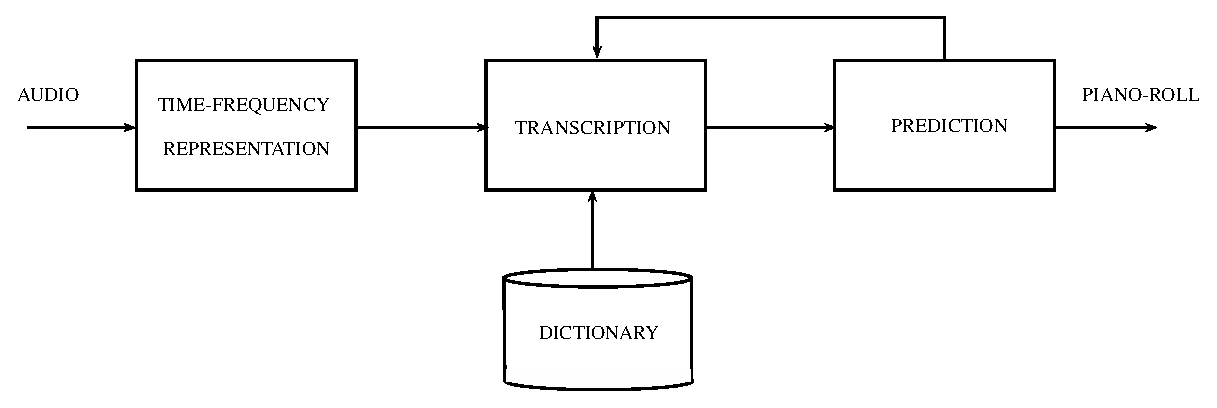
\includegraphics{figures/FigSystem.eps} 
 }
 \caption{Proposed system diagram.}
 \end{center}
 \vspace{-0.1in}
 \label{fig:system}
\end{figure*}


\section{Evaluation} \label{sec:evaluation}

\subsection{Dataset}

For testing the transcription system, we employ the Bach10 dataset \cite{Duan2010}, which is a freely available multi-track collection of multiple-instrument polyphonic music. It consists of ten recordings of J.S. Bach chorales, performed by violin, clarinet, saxophone, and bassoon. Pitch ground truth for each instrument is also provided. Due to the tonal and homogeneous content of the dataset (single composer, single music language), it is suitable for testing the incorporation of music language models in a multiple-instrument transcription system. For training the transcription system, pre-extracted and pre-shifted spectral templates are extracted for the instruments present in the dataset, using isolated note samples from the RWC database \cite{Goto2003}. 

For training the MLMs we use the Nottingham dataset\footnote{ifdo.ca/$\sim$seymour/nottingham/nottingham.html}, a collection of 1200 music pieces in symbolic ABC format, which contain simple chord combinations and tunes. We trained the RNN and the RNN-NADE models using both Stochastic Gradient Descent (SGD) and HF to compare performance. The inputs to both the models are sequences of length 200 where each frame of the sequence is a binary vector of length 88 which covers the full piano note range. We train both the RNN and the RNN-NADE to predict the next vector given a sequence of input vectors. We train the models by minimizing the negative log-likelihood of the sequences using the cross-entropy $ \sum_{i}t_{i}\log p_{i} + (1 - t_{i})\log(1-p_{i})$ where $i$ sums over all the dimensions of the binary vector and $t_i$ is the pitch target.


\subsection{Metrics}


For evaluating the performance of the proposed system for multi-pitch detection, we employ the precision ($\mathit{Pre}$), recall ($\mathit{Rec}$), and F-measure ($\mathit{F}$) metrics, which are commonly used in transcription evaluations \cite{MIREX}.
%\begin{equation}
% \mathit{Pre} = \frac{N_{\mathit{tp}}}{N_{\mathit{sys}}},\ \
%\ \mathit{Rec} = \frac{N_{\mathit{tp}}}{N_{\mathit{ref}}},\
%\ \ \mathit{F} = \frac{2\cdot\mathit{Rec}\cdot\mathit{Pre}}{\mathit{Rec}+\mathit{Pre}}
%\label{eq:PRF}
%\end{equation}
%where $N_{\mathit{tp}}$ is the number of correctly detected pitches, $N_{\mathit{sys}}$ is the number of detected pitches, and $N_{\mathit{ref}}$ is the number of ground-truth pitches. 
As in the public evaluations on multi-pitch detection carried out through the MIREX framework \cite{MIREX}, a detected note is considered correct if its pitch is the same as the ground truth pitch and its onset is within a 50ms tolerance interval of the ground-truth onset.

\subsection{Results}

To validate the performance of the MLMs, we calculate the prediction precision on unseen sequences of music from the Nottingham dataset of folk melodies. We utilise 694 tracks for training, 173 tracks for validation and 170 for testing\footnote{http://www-etud.iro.umontreal.ca/~boulanni/icml2012}. For both the RNN and RNN-NADE models we sample 10 vectors from the conditional distribution at each time-step and calculate the expected precision against the ground truth. The reported precision is found by finding the mean over the predictions of every frame. Table \ref{tab:prediction} shows the results of the validation experiments. These results are of the same order as the prediction accuracies reported in \cite{Boulanger-Lewandowski2012}. We found that for both the models, HF optimization gave better precision than SGD. Training with HF was also easier as there were less hyper parameters to be tuned when compared 
to SGD, where learning rate needs to be updated to make sure training is effective. The RNN models had a hidden layer of size 150, while the RNN-NADE models had a hidden layer of size 100 and the NADE consisted of a hidden layer of size 150. 

\begin{table}[t]
 \begin{center}
 \resizebox{150pt}{!}{
 \begin{tabular}{|l|c|}
  \hline
  \textbf{Model} & $\mathit{Pre}$ \\ \hline 
  RNN (SGD)  & 67.89\% \\ \hline
  RNN (HF) & 69.61\% \\ \hline
  RNN-NADE (SGD) & 68.89\% \\ \hline
  RNN-NADE (HF)  & \textbf{70.61}\% \\ \hline
     
 \end{tabular}
 }
\end{center}
 \caption{Validation results for MLMs}
 \label{tab:prediction}
\end{table}


Multi-pitch detection experiments are performed using the proposed system, with various configurations. A first configuration only considers the transcription system from Section \ref{sec:transcription}. A second configuration takes the output of the transcription system and gives it as input to the prediction system of Section \ref{sec:prediction}, where the final piano-roll is the output of the prediction step. A third configuration (presented in Section \ref{sec:combination}), re-transcribes the recording, having the prediction as a prior information for estimating the pitch activations. For the prediction system, experiments were performed using both the RNN-NADE and the RNN.

Results using the various system configurations are displayed in Table \ref{tab:results}. It can be seen that the best performance is achieved by the 3rd configuration when using the NADE-HF model for prediction, which surpasses the acoustic-only transcription system by more than 3\%. In general, it can be seen that using the prediction system as a post-processing step (2nd configuration) always leads to an improvement over the acoustic-only model (1st configuration). A similar trend can be observed when integrating the prediction information as a prior in the transcription system (configuration 3) compared to just using the prediction system as post-processing (configuration 2); an improvement is always reported. Another observation can be made when comparing the RNN-NADE with the RNN, with the former providing a clear improvement. For comparative purposes, we also trained MLMs using 500 MIDI files of J.S. Bach chorales\footnote{http://www.jsbchorales.net/sets.shtml} and tested the models on the Bach10 recordings. Using the Bach MLMs, the system reached $F =  63.58\%$, which is an improvement over the acoustic-only system, but is outperformed by the Nottingham language model. 

Qualitatively, the MLMs are able to improve transcription performance by providing a rough estimate of which pitches are expected to appear in the recording (and which pitches are not expected to appear). The language models were trained using simple chord sequences (from the Nottingham dataset) that are representative of simple tonal music and are applicable as language models to the more complex Bach chorales. We believe that the reason for the J.S. Bach MLMs not performing as well as the Nottingham MLMs is due to the fact that predicting Bach's music is a complex task (many exceptions, key changes, modulations), whereas a simple tonal model like the Nottingham dataset can work as a general-purpose language model in many types of music (this is also verified in \cite{Boulanger-Lewandowski2012}).

As an example of the proposed system's performance, the spectrogram and raw output of the system using the 3rd configuration is displayed for a recording from the Bach10 dataset in Fig. \ref{fig:Spectrogram}, whereas the post-processed transcription output along with the ground truth for the same recording is shown in Fig. \ref{fig:Transcription}.

By comparing with the method of \cite{Duan2010} (where the Bach10 dataset was first introduced), the proposed method using the frame-based accuracy metric which is defined in the same paper by Duan et al., reaches 74.3\% for the NADE-HF using the 3rd configuration, whereas the method of \cite{Duan2010} reaches 69.7\% (with unknown polyphony).

\begin{table}[t]
 \begin{center}
 \resizebox{230pt}{!}{
 \begin{tabular}{|l|c|c|c|}
  \hline
  \textbf{Configuration} & $\mathit{F}$ & $\mathit{Pre}$ & $\mathit{Rec}$  \\ \hline 
  Configuration 1 & 62.02\%  & 58.51\% & 66.12\% \\ \hline
  Configuration 2 - NADE & 62.62\% & 59.70\% & 65.92\% \\ \hline
  Configuration 3 - NADE & 64.08\% & 61.96\% & 66.44\% \\ \hline
  Configuration 2 - RNN & 62.29\% & 59.08\% & 65.98\% \\ \hline
  Configuration 3 - RNN & 63.85\% & 61.14\% & 66.90\% \\ \hline  
  Configuration 2 - NADE-HF & 62.20\% & 59.14\% & 65.68\% \\ \hline
  Configuration 3 - NADE-HF & \textbf{65.16}\% & \textbf{62.80}\% & \textbf{67.78}\% \\ \hline  
  Configuration 2 - RNN-HF & 62.44\% & 59.28\% & 66.07\% \\ \hline
  Configuration 3 - RNN-HF & 62.87\% & 60.03\% & 66.11\% \\ \hline    
 \end{tabular}
 }
\end{center}
\vspace{-0.1in}
 \caption{Transcription results using various system configurations.}
 \label{tab:results}
\end{table}


\begin{figure}[t]
 \resizebox{230pt}{!}{
 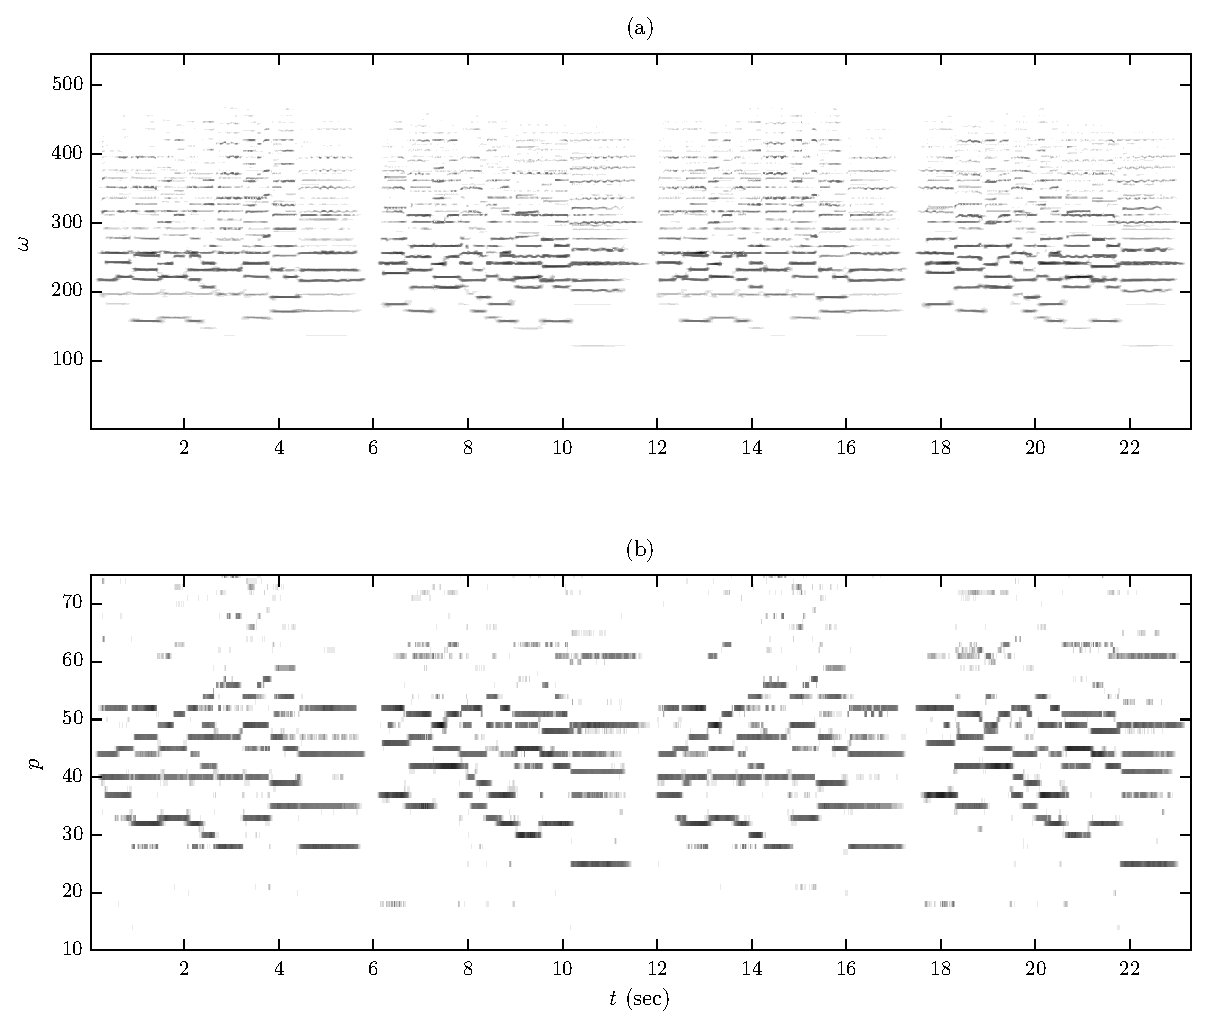
\includegraphics{figures/FigSpectrogram.eps}
 }
 \vspace{-0.05in}
 \caption{(a) The spectrogram $V_{\omega,t}$ for recording ``Ach Lieben Christen'' from the Bach10 dataset. (b) The pitch activation $P(p,t)$ using the  transcription-prediction system using the 3rd configuration, with the NADE-HF.}
 \label{fig:Spectrogram}
\end{figure}

\begin{figure}[t]
 \resizebox{230pt}{!}{
 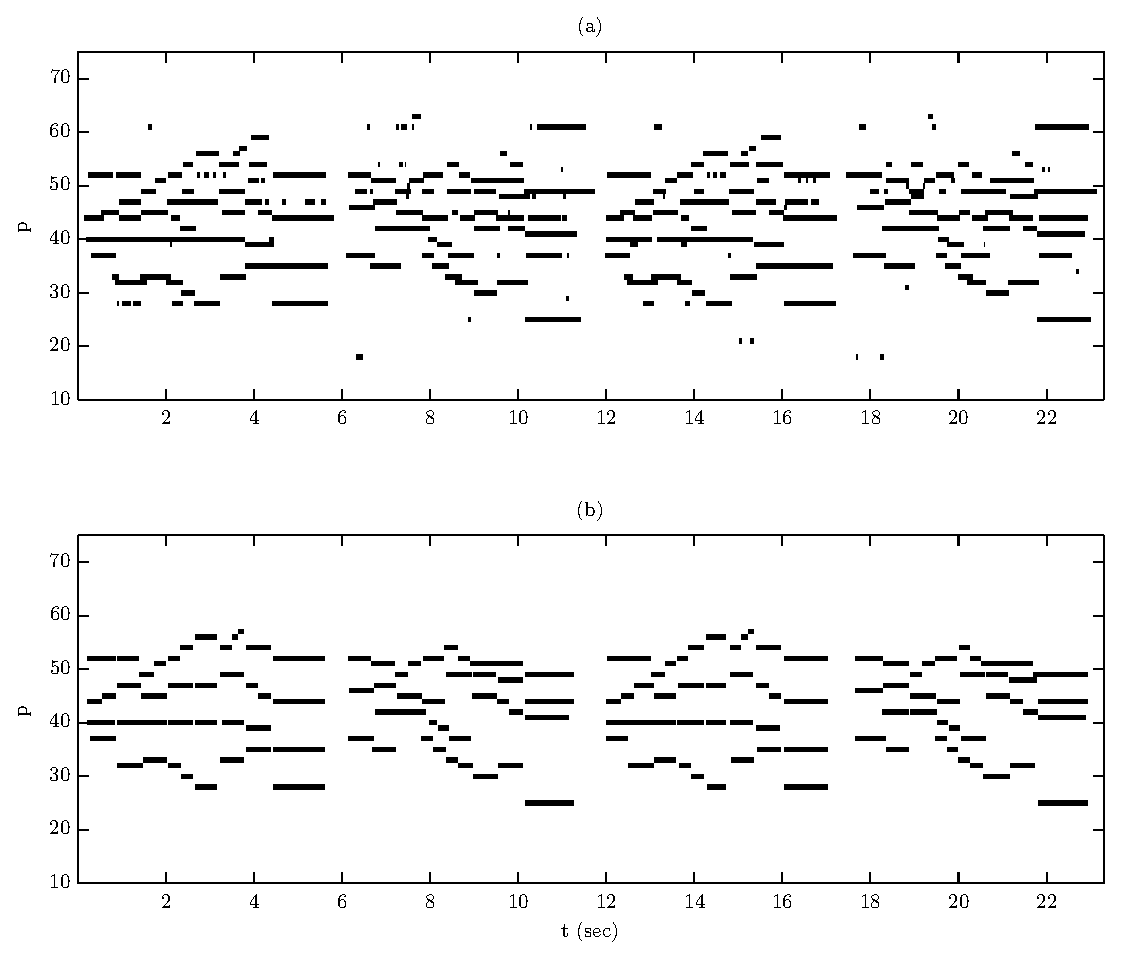
\includegraphics{figures/FigTranscription.eps}
 }
  \vspace{-0.05in}
 \caption{Transcription example for recording ``Ach Lieben Christen'' from the Bach10 dataset. (a) The post-processed output of the transcription-predicton system using the 3rd configuration, with the NADE-HF. (b) The pitch ground truth of the recording.}
 \label{fig:Transcription}
\end{figure}



\section{Conclusions} \label{sec:conclusions}

In this paper, we proposed a system for automatic music transcription which incorporated prior information from a polyphonic music prediction model based on recurrent neural networks. The acoustic transcription model was based on probabilistic latent component analysis, and information from the prediction system was incorporated using Dirichlet priors. Experimental results using the multiple-instrument Bach10 dataset showed that there is a clear and significant improvement (3\% in terms of F-measure) by combining a music language model with an acoustic model for improving the performance of the latter. These results also demonstrate that the MLM can be trained on symbolic music data from a different source as the acoustic data, thus eliminating the need to acquire collections of symbolic and corresponding acoustic data (which are scarce).

In the current system, the language models are trained  on only one dataset. In the future, we would like to evaluate the proposed system using language models trained from different sources to see if this helps the MLMs generalize better. We will also investigate different system configurations, to test whether iterating the transcription and prediction steps leads to improved performance. We will also investigate the effect of using different RNN architectures like Long Short Term Memory (LSTM) and bi-directional RNNs and LSTMs. Finally, we would like to extend and improve the current models for high-dimensional sequences to better fit the requirements for music language modelling. 

\bibliography{bibliography}

%\bibliography{ismir2014template}

\end{document}
